\documentclass[twoside]{book}

% Packages required by doxygen
\usepackage{fixltx2e}
\usepackage{calc}
\usepackage{doxygen}
\usepackage[export]{adjustbox} % also loads graphicx
\usepackage{graphicx}
\usepackage[utf8]{inputenc}
\usepackage{makeidx}
\usepackage{multicol}
\usepackage{multirow}
\PassOptionsToPackage{warn}{textcomp}
\usepackage{textcomp}
\usepackage[nointegrals]{wasysym}
\usepackage[table]{xcolor}

% Font selection
\usepackage[T1]{fontenc}
\usepackage[scaled=.90]{helvet}
\usepackage{courier}
\usepackage{amssymb}
\usepackage{sectsty}
\renewcommand{\familydefault}{\sfdefault}
\allsectionsfont{%
  \fontseries{bc}\selectfont%
  \color{darkgray}%
}
\renewcommand{\DoxyLabelFont}{%
  \fontseries{bc}\selectfont%
  \color{darkgray}%
}
\newcommand{\+}{\discretionary{\mbox{\scriptsize$\hookleftarrow$}}{}{}}

% Page & text layout
\usepackage{geometry}
\geometry{%
  a4paper,%
  top=2.5cm,%
  bottom=2.5cm,%
  left=2.5cm,%
  right=2.5cm%
}
\tolerance=750
\hfuzz=15pt
\hbadness=750
\setlength{\emergencystretch}{15pt}
\setlength{\parindent}{0cm}
\setlength{\parskip}{3ex plus 2ex minus 2ex}
\makeatletter
\renewcommand{\paragraph}{%
  \@startsection{paragraph}{4}{0ex}{-1.0ex}{1.0ex}{%
    \normalfont\normalsize\bfseries\SS@parafont%
  }%
}
\renewcommand{\subparagraph}{%
  \@startsection{subparagraph}{5}{0ex}{-1.0ex}{1.0ex}{%
    \normalfont\normalsize\bfseries\SS@subparafont%
  }%
}
\makeatother

% Headers & footers
\usepackage{fancyhdr}
\pagestyle{fancyplain}
\fancyhead[LE]{\fancyplain{}{\bfseries\thepage}}
\fancyhead[CE]{\fancyplain{}{}}
\fancyhead[RE]{\fancyplain{}{\bfseries\leftmark}}
\fancyhead[LO]{\fancyplain{}{\bfseries\rightmark}}
\fancyhead[CO]{\fancyplain{}{}}
\fancyhead[RO]{\fancyplain{}{\bfseries\thepage}}
\fancyfoot[LE]{\fancyplain{}{}}
\fancyfoot[CE]{\fancyplain{}{}}
\fancyfoot[RE]{\fancyplain{}{\bfseries\scriptsize Generated by Doxygen }}
\fancyfoot[LO]{\fancyplain{}{\bfseries\scriptsize Generated by Doxygen }}
\fancyfoot[CO]{\fancyplain{}{}}
\fancyfoot[RO]{\fancyplain{}{}}
\renewcommand{\footrulewidth}{0.4pt}
\renewcommand{\chaptermark}[1]{%
  \markboth{#1}{}%
}
\renewcommand{\sectionmark}[1]{%
  \markright{\thesection\ #1}%
}

% Indices & bibliography
\usepackage{natbib}
\usepackage[titles]{tocloft}
\setcounter{tocdepth}{3}
\setcounter{secnumdepth}{5}
\makeindex

% Hyperlinks (required, but should be loaded last)
\usepackage{ifpdf}
\ifpdf
  \usepackage[pdftex,pagebackref=true]{hyperref}
\else
  \usepackage[ps2pdf,pagebackref=true]{hyperref}
\fi
\hypersetup{%
  colorlinks=true,%
  linkcolor=blue,%
  citecolor=blue,%
  unicode%
}

% Custom commands
\newcommand{\clearemptydoublepage}{%
  \newpage{\pagestyle{empty}\cleardoublepage}%
}

\usepackage{caption}
\captionsetup{labelsep=space,justification=centering,font={bf},singlelinecheck=off,skip=4pt,position=top}

%===== C O N T E N T S =====

\begin{document}

% Titlepage & ToC
\hypersetup{pageanchor=false,
             bookmarksnumbered=true,
             pdfencoding=unicode
            }
\pagenumbering{alph}
\begin{titlepage}
\vspace*{7cm}
\begin{center}%
{\Large Dyn\+Rup \\[1ex]\large 0.\+1 }\\
\vspace*{1cm}
{\large Generated by Doxygen 1.8.14}\\
\end{center}
\end{titlepage}
\clearemptydoublepage
\pagenumbering{roman}
\tableofcontents
\clearemptydoublepage
\pagenumbering{arabic}
\hypersetup{pageanchor=true}

%--- Begin generated contents ---
\chapter{Hierarchical Index}
\section{Class Hierarchy}
This inheritance list is sorted roughly, but not completely, alphabetically\+:\begin{DoxyCompactList}
\item \contentsline{section}{Element}{\pageref{class_element}}{}
\begin{DoxyCompactList}
\item \contentsline{section}{Quad4\+\_\+\+Element}{\pageref{class_quad4___element}}{}
\end{DoxyCompactList}
\item \contentsline{section}{Mesh}{\pageref{class_mesh}}{}
\item \contentsline{section}{xind$<$ T $>$}{\pageref{classxind}}{}
\end{DoxyCompactList}

\chapter{Class Index}
\section{Class List}
Here are the classes, structs, unions and interfaces with brief descriptions\+:\begin{DoxyCompactList}
\item\contentsline{section}{\mbox{\hyperlink{class_element}{Element}} }{\pageref{class_element}}{}
\item\contentsline{section}{\mbox{\hyperlink{class_mesh}{Mesh}} }{\pageref{class_mesh}}{}
\item\contentsline{section}{\mbox{\hyperlink{class_quad4___element}{Quad4\+\_\+\+Element}} }{\pageref{class_quad4___element}}{}
\item\contentsline{section}{\mbox{\hyperlink{classxind}{xind$<$ T $>$}} }{\pageref{classxind}}{}
\end{DoxyCompactList}

\chapter{Class Documentation}
\hypertarget{class_element}{}\section{Element Class Reference}
\label{class_element}\index{Element@{Element}}
Inheritance diagram for Element\+:\begin{figure}[H]
\begin{center}
\leavevmode
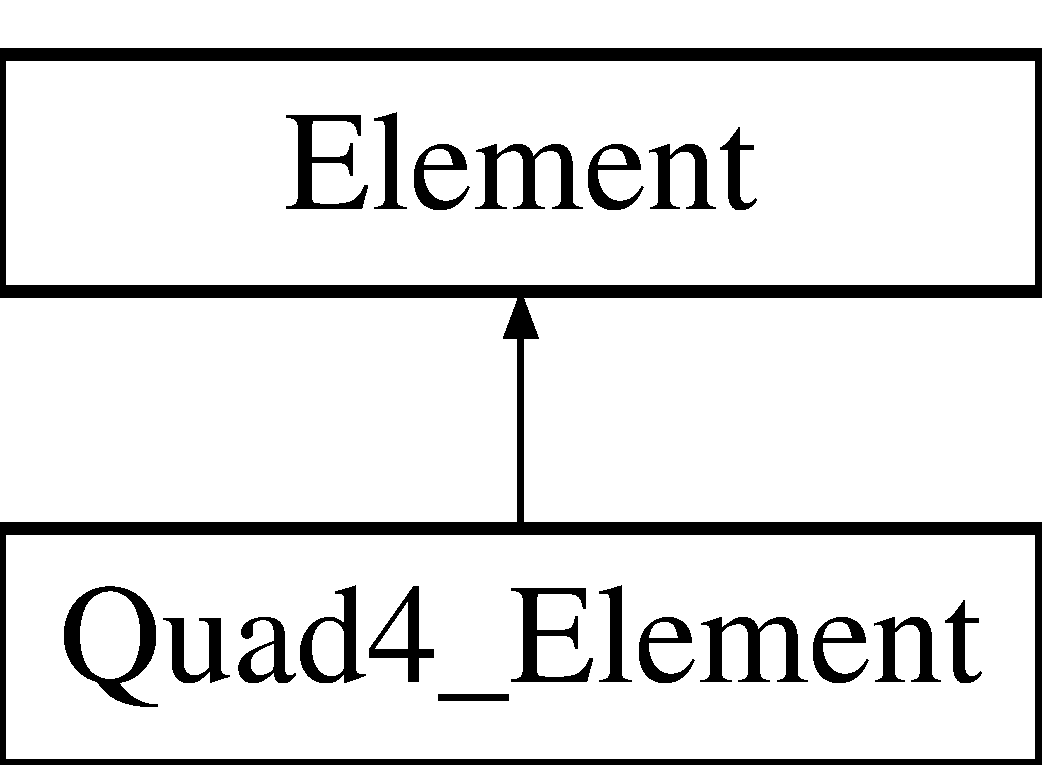
\includegraphics[height=2.000000cm]{class_element}
\end{center}
\end{figure}
\subsection*{Public Member Functions}
\begin{DoxyCompactItemize}
\item 
\mbox{\hyperlink{class_element_ab0d0e20be9a36ae676202db753faeec9}{Element}} ()
\end{DoxyCompactItemize}
\subsection*{Protected Member Functions}
\begin{DoxyCompactItemize}
\item 
\mbox{\Hypertarget{class_element_a6d39782237857b49ef63d8e7a0c4f4c3}\label{class_element_a6d39782237857b49ef63d8e7a0c4f4c3}} 
virtual void {\bfseries cal\+\_\+ke} ()=0
\end{DoxyCompactItemize}
\subsection*{Protected Attributes}
\begin{DoxyCompactItemize}
\item 
\mbox{\Hypertarget{class_element_ade82c5d130fa5828e3d52c4065a36b85}\label{class_element_ade82c5d130fa5828e3d52c4065a36b85}} 
Array\+X\+X\+S\+RM {\bfseries ke}
\end{DoxyCompactItemize}


\subsection{Detailed Description}


Definition at line 23 of file Element.\+h.



\subsection{Constructor \& Destructor Documentation}
\mbox{\Hypertarget{class_element_ab0d0e20be9a36ae676202db753faeec9}\label{class_element_ab0d0e20be9a36ae676202db753faeec9}} 
\index{Element@{Element}!Element@{Element}}
\index{Element@{Element}!Element@{Element}}
\subsubsection{\texorpdfstring{Element()}{Element()}}
{\footnotesize\ttfamily Element\+::\+Element (\begin{DoxyParamCaption}{ }\end{DoxyParamCaption})}

Default constructor 

Definition at line 8 of file Element.\+cc.


\begin{DoxyCode}
9 \{
10     std::cout<<\textcolor{stringliteral}{"haha\_ELement"}<<std::endl;
11 \}
\end{DoxyCode}


The documentation for this class was generated from the following files\+:\begin{DoxyCompactItemize}
\item 
include/Element.\+h\item 
src/Element.\+cc\end{DoxyCompactItemize}

\hypertarget{class_mesh}{}\section{Mesh Class Reference}
\label{class_mesh}\index{Mesh@{Mesh}}
\subsection*{Public Member Functions}
\begin{DoxyCompactItemize}
\item 
\mbox{\hyperlink{class_mesh_a2af137f1571af89172b9c102302c416b}{Mesh}} ()
\item 
Petsc\+Error\+Code \mbox{\hyperlink{class_mesh_aa381581e1c9fe95f438d4a66c4291a5f}{Abaqus\+\_\+\+IO}} (std\+::string \&fname)
\item 
Petsc\+Error\+Code \mbox{\hyperlink{class_mesh_a69a626f34e07b13615847d2d3028f20b}{Redistribute}} ()
\end{DoxyCompactItemize}
\subsection*{Public Attributes}
\begin{DoxyCompactItemize}
\item 
\mbox{\Hypertarget{class_mesh_ae30b0028e49c22ae7a6fff0a89db7394}\label{class_mesh_ae30b0028e49c22ae7a6fff0a89db7394}} 
M\+P\+I\+\_\+\+Comm {\bfseries comm}
\item 
\mbox{\Hypertarget{class_mesh_ab4d9d2c7e02931d2d803da95516eaa20}\label{class_mesh_ab4d9d2c7e02931d2d803da95516eaa20}} 
int {\bfseries myid}
\item 
\mbox{\Hypertarget{class_mesh_a8a2f6f435dc9166168d2cda553d833e7}\label{class_mesh_a8a2f6f435dc9166168d2cda553d833e7}} 
int {\bfseries nprocs}
\item 
\mbox{\Hypertarget{class_mesh_ab7f1c680291e263a5b83eec2796b9923}\label{class_mesh_ab7f1c680291e263a5b83eec2796b9923}} 
Petsc\+Int {\bfseries n\+Dims}
\item 
\mbox{\Hypertarget{class_mesh_a1160f45b158032295a5dde423d3b782a}\label{class_mesh_a1160f45b158032295a5dde423d3b782a}} 
Array\+X\+X\+S\+RM {\bfseries Node}
\item 
\mbox{\Hypertarget{class_mesh_ad4f5557e8d2104647a235669f8df09cd}\label{class_mesh_ad4f5557e8d2104647a235669f8df09cd}} 
Array\+X\+X\+I\+RM {\bfseries Element}
\item 
\mbox{\Hypertarget{class_mesh_ae9d1873e57dc7cb666329946c29bbd1b}\label{class_mesh_ae9d1873e57dc7cb666329946c29bbd1b}} 
Array\+XI {\bfseries g\+Elem}
\item 
\mbox{\Hypertarget{class_mesh_a11aa956306c304ccfa37572de291c705}\label{class_mesh_a11aa956306c304ccfa37572de291c705}} 
Array\+XI {\bfseries g\+Node}
\item 
\mbox{\Hypertarget{class_mesh_a1d49421b1ab9aadd6ff11a9caf8de819}\label{class_mesh_a1d49421b1ab9aadd6ff11a9caf8de819}} 
Array\+XI {\bfseries el\+Dist}
\item 
\mbox{\Hypertarget{class_mesh_a6ce034f24bd0d73310649991f5374d13}\label{class_mesh_a6ce034f24bd0d73310649991f5374d13}} 
Array\+XI {\bfseries nd\+Dist}
\item 
\mbox{\Hypertarget{class_mesh_ae1ba84601920b113eba2f99adbaca2d4}\label{class_mesh_ae1ba84601920b113eba2f99adbaca2d4}} 
Petsc\+Int {\bfseries n\+Elem}
\item 
\mbox{\Hypertarget{class_mesh_a2e5ff5315bd999af1361e6afe7a78ed6}\label{class_mesh_a2e5ff5315bd999af1361e6afe7a78ed6}} 
Petsc\+Int {\bfseries n\+Node}
\item 
\mbox{\Hypertarget{class_mesh_af1953886f04ff875c2ca36da8a4f38e2}\label{class_mesh_af1953886f04ff875c2ca36da8a4f38e2}} 
Petsc\+Int {\bfseries n\+Loc\+Elem}
\item 
\mbox{\Hypertarget{class_mesh_a9f1050136cf607064480c079976a6663}\label{class_mesh_a9f1050136cf607064480c079976a6663}} 
Petsc\+Int {\bfseries n\+Loc\+Node}
\item 
\mbox{\Hypertarget{class_mesh_a3f9917990c7eab0ec45e48131737acf1}\label{class_mesh_a3f9917990c7eab0ec45e48131737acf1}} 
Vec {\bfseries U}
\item 
\mbox{\Hypertarget{class_mesh_a7a473f5eda4af43fb9d83873c51f52b0}\label{class_mesh_a7a473f5eda4af43fb9d83873c51f52b0}} 
Vec {\bfseries F}
\end{DoxyCompactItemize}
\subsection*{Protected Member Functions}
\begin{DoxyCompactItemize}
\item 
Petsc\+Error\+Code \mbox{\hyperlink{class_mesh_a0ab1f20471ff5deed8803597b979779d}{Reorder\+M\+E\+T\+IS}} (Petsc\+Int nparts=0, Petsc\+Int ncommon\+Nodes=0, Petsc\+Scalar $\ast$tpwgts=N\+U\+LL, Petsc\+Int $\ast$elmwgt=N\+U\+LL, Petsc\+Int $\ast$opts=N\+U\+LL)
\item 
Petsc\+Error\+Code \mbox{\hyperlink{class_mesh_ab9c61b0cf7cbcb8738d0e904fe532e91}{Reorder\+Par\+M\+E\+T\+IS}} (Petsc\+Int nparts=0, Petsc\+Int ncommon\+Nodes=0, Petsc\+Scalar $\ast$tpwgts=N\+U\+LL, Petsc\+Scalar $\ast$ubvec=N\+U\+LL, Petsc\+Int $\ast$opts=N\+U\+LL, Petsc\+Int ncon=1, Petsc\+Int $\ast$elmwgt=N\+U\+LL, Petsc\+Int wgtflag=0, Petsc\+Int numflag=0)
\item 
Petsc\+Error\+Code \mbox{\hyperlink{class_mesh_a1c915802d56c4ded24e460e83cfb5399}{Elem\+Dist}} (Eigen\+::\+Array$<$ Petsc\+Int, -\/1, 1 $>$ \&partition)
\item 
Petsc\+Error\+Code \mbox{\hyperlink{class_mesh_aa6b19f4fdf210f8937694e8c7d30ea15}{Node\+Dist}} ()
\item 
Petsc\+Error\+Code \mbox{\hyperlink{class_mesh_a1930d80c707de6d202dac7cef0022257}{Expand\+\_\+\+Node}} ()
\item 
Petsc\+Error\+Code \mbox{\hyperlink{class_mesh_af9e180bd8adb9c495e6c38840ea19f10}{Initialize\+\_\+\+Vectors}} ()
\item 
Petsc\+Error\+Code \mbox{\hyperlink{class_mesh_a54a12376bf99f4f4991af01fc23c9c09}{Localize}} ()
\end{DoxyCompactItemize}


\subsection{Detailed Description}


Definition at line 21 of file mesh.\+h.



\subsection{Constructor \& Destructor Documentation}
\mbox{\Hypertarget{class_mesh_a2af137f1571af89172b9c102302c416b}\label{class_mesh_a2af137f1571af89172b9c102302c416b}} 
\index{Mesh@{Mesh}!Mesh@{Mesh}}
\index{Mesh@{Mesh}!Mesh@{Mesh}}
\subsubsection{\texorpdfstring{Mesh()}{Mesh()}}
{\footnotesize\ttfamily Mesh\+::\+Mesh (\begin{DoxyParamCaption}{ }\end{DoxyParamCaption})}

Default constructor 

Definition at line 14 of file mesh.\+cc.


\begin{DoxyCode}
15 \{
16   comm = MPI\_COMM\_WORLD;
17   MPI\_Comm\_rank(comm, &myid);
18   MPI\_Comm\_size(comm, &nprocs);
19 \}
\end{DoxyCode}


\subsection{Member Function Documentation}
\mbox{\Hypertarget{class_mesh_aa381581e1c9fe95f438d4a66c4291a5f}\label{class_mesh_aa381581e1c9fe95f438d4a66c4291a5f}} 
\index{Mesh@{Mesh}!Abaqus\+\_\+\+IO@{Abaqus\+\_\+\+IO}}
\index{Abaqus\+\_\+\+IO@{Abaqus\+\_\+\+IO}!Mesh@{Mesh}}
\subsubsection{\texorpdfstring{Abaqus\+\_\+\+I\+O()}{Abaqus\_IO()}}
{\footnotesize\ttfamily Petsc\+Error\+Code Mesh\+::\+Abaqus\+\_\+\+IO (\begin{DoxyParamCaption}\item[{std\+::string \&}]{fname }\end{DoxyParamCaption})}

Read in Abaqus mesh 

Definition at line 24 of file mesh.\+cc.


\begin{DoxyCode}
25 \{
26   PetscErrorCode err = 0;
27   \textcolor{keywordflow}{if} (myid == 0)
28   \{
29     std::string s;
30     std::ifstream \_in(fname);
31     \textcolor{keywordflow}{while} (\textcolor{keyword}{true})
32     \{
33       std::getline(\_in,s);
34       \textcolor{comment}{// Convert s to uppercase}
35       std::string upper(s);
36       std::transform(upper.begin(), upper.end(), upper.begin(), ::toupper);
37       \textcolor{comment}{// 0.) Look for the "*Part" Section}
38 \textcolor{comment}{//      if (upper.find("*PART")== static\_cast<std::string::size\_type>(0))}
39 \textcolor{comment}{//      \{}
40 \textcolor{comment}{//        std::cout<<"Find *PART"<<std::endl;}
41 \textcolor{comment}{//      \}}
42       \textcolor{comment}{// 1.) Loop for the "*Nodes" section}
43       \textcolor{keywordflow}{if} (upper.find(\textcolor{stringliteral}{"*NODE"})== \textcolor{keyword}{static\_cast<}std::string::size\_type\textcolor{keyword}{>}(0))
44       \{
45         \textcolor{comment}{//std::string nset\_name = s ;}
46         \textcolor{comment}{//std::cout<<s<<std::endl;}
47         \textcolor{comment}{// Temperatry variables for parsing lines of text}
48         \textcolor{keywordtype}{char} c ;
49         std::string line;
50         \textcolor{keywordtype}{int} i=0;
51         \textcolor{keywordflow}{while} (\_in.peek()!=\textcolor{charliteral}{'*'}&&\_in.peek()!=EOF)
52         \{
53           \textcolor{comment}{// Read an entire line which corresponds to a single points's id and (x,y) value}
54           std::getline(\_in,line);
55           \textcolor{comment}{// Revomie all whitesspaces characters from the line}
56           line.erase(std::remove\_if(line.begin(),line.end(),::isspace),line.end());
57           \textcolor{comment}{// Make a stream out of the modified line so we can stream values from it in the usaly way}
58           std::stringstream ss(line);
59           \textcolor{keywordtype}{int} abaqus\_Node\_id = 0;
60           \textcolor{keywordtype}{double} x = 0 , y = 0;
61           ss >> abaqus\_Node\_id >> c >> x >>c >> y ;
62           Node.conservativeResize(i+1, 2);
63           Node.row(i)<< x , y ;
64           i++;
65         \}
66         \textcolor{comment}{//  std::cout<< Nodes<< "\(\backslash\)n"<< Nodes.rows()<<std::endl;}
67       \}
68       \textcolor{keywordflow}{else} \textcolor{keywordflow}{if} (upper.find(\textcolor{stringliteral}{"*ELEMENT,"})==\textcolor{keyword}{static\_cast<}std::string::size\_type\textcolor{keyword}{>}(0))
69       \{
70         \textcolor{comment}{//std::string elset\_name = s;}
71         \textcolor{comment}{//std::cout<<s <<std::endl;}
72         \textcolor{keywordtype}{char} c ;
73         std::string line;
74         \textcolor{keywordtype}{int} i = 0;
75         \textcolor{keywordflow}{while} (\_in.peek()!=\textcolor{charliteral}{'*'}&&\_in.peek()!=EOF)
76         \{
77           \textcolor{comment}{// Read an entire line which corresponds to a single Element's id and connectivity value
       (Q4\_only)}
78           std::getline(\_in,line);
79           \textcolor{comment}{// Revomie all whitesspaces characters from the line}
80           line.erase(std::remove\_if(line.begin(),line.end(),::isspace),line.end());
81           \textcolor{comment}{// Make a stream out of the modified line so we can stream values from it in the usaly way}
82           std::stringstream ss(line);
83           \textcolor{keywordtype}{int} abaqus\_el\_id = 0;
84           \textcolor{keywordtype}{int} Node1 =0 , Node2 =0 , Node3 = 0 , Node4 =0;
85           ss >> abaqus\_el\_id >> c >> Node1 >> c >>Node2 >> c >> Node3 >> c >> Node4 ;
86           \textcolor{comment}{// add -1 here becasue we are using a zero Node numbering zero is the first Node}
87           Element.conservativeResize(i+1, 4);
88           Element.row(i)<<Node1-1,Node2-1,Node3-1,Node4-1;
89           i++;
90         \}
91       \}
92       \textcolor{keywordflow}{if} (\_in.eof())
93         \textcolor{keywordflow}{break};
94     \}
95 
96     \textcolor{comment}{// Set distribution variables}
97     nLocElem = Element.rows();
98     nLocNode = Node.rows();
99     elDist.setConstant(nprocs+1, nLocElem);
100     ndDist.setConstant(nprocs+1, nLocNode);
101     elDist(0) = 0;
102     ndDist(0) = 0;
103   \}
104   \textcolor{keywordflow}{else}
105   \{
106     \textcolor{comment}{// Set distribution variables}
107     nLocElem = 0;
108     nLocNode = 0;
109     elDist.resize(nprocs+1);
110     ndDist.resize(nprocs+1);
111   \}
112 
113   \textcolor{comment}{// Distribute Element and Node distribution arrays}
114   err = MPI\_Bcast(elDist.data(), nprocs+1, MPI\_INT, 0, comm);
115   err = MPI\_Bcast(ndDist.data(), nprocs+1, MPI\_INT, 0, comm);
116   nElem = elDist(nprocs);
117   nNode = ndDist(nprocs);
118   nDims = 2; \textcolor{comment}{// TODO generalize this to ND meshes}
119 
120   \textcolor{keywordflow}{return} err;
121 \}
\end{DoxyCode}
\mbox{\Hypertarget{class_mesh_a1c915802d56c4ded24e460e83cfb5399}\label{class_mesh_a1c915802d56c4ded24e460e83cfb5399}} 
\index{Mesh@{Mesh}!Elem\+Dist@{Elem\+Dist}}
\index{Elem\+Dist@{Elem\+Dist}!Mesh@{Mesh}}
\subsubsection{\texorpdfstring{Elem\+Dist()}{ElemDist()}}
{\footnotesize\ttfamily Petsc\+Error\+Code Mesh\+::\+Elem\+Dist (\begin{DoxyParamCaption}\item[{Eigen\+::\+Array$<$ Petsc\+Int, -\/1, 1 $>$ \&}]{partition }\end{DoxyParamCaption})\hspace{0.3cm}{\ttfamily [protected]}}

Redistribute Elements Reallocate Elements Note abbreviations\+: senddisp = first Element in array sent to each process sendcnt = how many Elements sent to each process -\/ TO BE R\+E\+M\+O\+V\+ED transfer\+Size = how many Elements each process is sending to the other processes recvcnt = how many Elements received from each process recvdsp = beginning location of buffer to receive Elements from each process elmcpy = a copy of Element reordered for continguous send buffers where = after initial sorting, the local number of each Element permute = permutation vector for filter matrix (global) 

Definition at line 297 of file mesh.\+cc.


\begin{DoxyCode}
298 \{
299   PetscErrorCode ierr = 0;
309   \textcolor{comment}{// Initialize transfer Variables}
310   \textcolor{keywordtype}{short} elementSize = pow(2,nDims);
311   ArrayXI where = EigLab::gensort(partition).cast<PetscInt>();
312   ArrayXXI transferSize = ArrayXXI::Zero(nprocs,nprocs);
313   ArrayXXIRM elmcpy(Element.rows(),Element.cols());
314   \textcolor{keywordflow}{for} (PetscInt i = 0; i < partition.rows(); i++)
315   \{
316     elmcpy.row(i) = Element.row(where(i));
317     transferSize(partition(i),myid)++;
318   \}
319 
320   \textcolor{comment}{// How many Elements are transferred between each pair of processes}
321   MPI\_Allgather(MPI\_IN\_PLACE, 0, MPIU\_INT, transferSize.data(),
322                 nprocs, MPIU\_INT, comm);
323   Eigen::ArrayXi sendcnt = elementSize*transferSize.col(myid).cast<\textcolor{keywordtype}{int}>();
324   Eigen::ArrayXi recvcnt = elementSize*transferSize.row(myid).cast<\textcolor{keywordtype}{int}>();
325 
326   \textcolor{comment}{// Offsets in sent messages}
327   Eigen::ArrayXi senddsp = Eigen::ArrayXi::Zero(nprocs);
328   \textcolor{keywordflow}{for} (\textcolor{keywordtype}{short} i = 1; i < nprocs; i++)
329     senddsp(i) = sendcnt(i-1) + senddsp(i-1);
330 
331   \textcolor{comment}{// Offsets in received messages}
332   Eigen::ArrayXi recvdsp = Eigen::ArrayXi::Zero(nprocs);
333   \textcolor{keywordflow}{for} (\textcolor{keywordtype}{short} i = 1; i < nprocs; i++)
334     recvdsp(i) = recvcnt(i-1) + recvdsp(i-1);
335 
336   \textcolor{comment}{// The Element transfer}
337   Element.resize(recvcnt.sum()/elementSize, elementSize);
338   MPI\_Alltoallv(elmcpy.data(), sendcnt.data(), senddsp.data(),
339                 MPIU\_INT, Element.data(), recvcnt.data(),
340                 recvdsp.data(), MPIU\_INT, comm);
341 
342   \textcolor{comment}{// Update distribution across processes}
343   elDist(myid+1) = Element.rows();
344   nLocElem = Element.rows();
345   MPI\_Allgather(MPI\_IN\_PLACE, 0, MPI\_DATATYPE\_NULL, elDist.data()+1,
346                 1, MPIU\_INT, comm);
347   \textcolor{keywordflow}{for} (\textcolor{keywordtype}{short} i = 1; i <= nprocs; i++)
348     elDist(i) += elDist(i-1);
349 
350   \textcolor{comment}{// Create global permutation array after sharing Elements}
351   \textcolor{comment}{// This is currently assembling a global vector on all processes and reducing}
352   \textcolor{comment}{// it.  The performance could possibly be improved by sharing the local parts}
353   \textcolor{comment}{// and then assembling after transfer, thereby reducing communications.}
354   \textcolor{comment}{// Permute = permutation vector, permute(i) = newi}
355   \textcolor{comment}{// Indices = vector indicating where this process can start assigning Elements}
356   \textcolor{comment}{//            on each process (i.e. global locations in the permute vector)}
357   ArrayXI permute = ArrayXI::Zero(nElem);
358   ArrayXI indices = ArrayXI::Zero(nprocs);
359   indices.segment(1,nprocs-1) = transferSize.block(0, 0, nprocs-1, nprocs)
360                                 .rowwise().sum();
361   partial\_sum(indices.data(), indices.data()+nprocs, indices.data());
362   indices += transferSize.block(0, 0, nprocs, myid).rowwise().sum();
363   \textcolor{keywordtype}{int} permuteStart = transferSize.block(0, 0, nprocs, myid).sum();
364   \textcolor{keywordflow}{for} (PetscInt i = 0; i < partition.rows(); i++)
365   \{
366     permute(where(i)+permuteStart) = indices(partition(i))++;
367   \}
368   MPI\_Allreduce(MPI\_IN\_PLACE, permute.data(), nElem, MPIU\_INT, MPI\_SUM, comm);
369 
370   \textcolor{keywordflow}{return} ierr;
371 \}
\end{DoxyCode}
\mbox{\Hypertarget{class_mesh_a1930d80c707de6d202dac7cef0022257}\label{class_mesh_a1930d80c707de6d202dac7cef0022257}} 
\index{Mesh@{Mesh}!Expand\+\_\+\+Node@{Expand\+\_\+\+Node}}
\index{Expand\+\_\+\+Node@{Expand\+\_\+\+Node}!Mesh@{Mesh}}
\subsubsection{\texorpdfstring{Expand\+\_\+\+Node()}{Expand\_Node()}}
{\footnotesize\ttfamily Petsc\+Error\+Code Mesh\+::\+Expand\+\_\+\+Node (\begin{DoxyParamCaption}{ }\end{DoxyParamCaption})\hspace{0.3cm}{\ttfamily [protected]}}

Capture surrounding Nodes on other processes List of all the Nodes the local Elements need

Pull out already owned Nodes

Find where all those Nodes are and how many Nodes are neede from each process

Tell each process how many Nodes you need sent over

Offsets in recieved messages regarding which Nodes are requested

Get offsets in sent messages requesting Nodes

Send the Nodes you want to each process

Pack up all the Nodes for sending

Ship the Nodes

Update the global Node list 

Definition at line 452 of file mesh.\+cc.


\begin{DoxyCode}
453 \{
454   PetscErrorCode ierr = 0;
455 
457   ArrayXI ndlist = Eigen::Map<ArrayXI>(Element.data(),Element.size());
458   EigLab::Unique(ndlist, 1);
459 
461   PetscInt ind = 0, nind = 0;
462   \textcolor{keywordflow}{for} (PetscInt i = 0; i < ndlist.rows(); i++)
463   \{
464       \textcolor{keywordflow}{if} (ind == gNode.size())
465       \{
466           ndlist.segment(nind, ndlist.rows()-i) = ndlist.segment(i, ndlist.rows()-i);
467           nind += ndlist.rows()-i;
468           \textcolor{keywordflow}{break};
469       \}
470       \textcolor{keywordflow}{if} (gNode(ind) != ndlist(i))
471           ndlist(nind++) = ndlist(i);
472       \textcolor{keywordflow}{else}
473           ind++;
474   \}
475   ndlist.conservativeResize(nind);
476 
478   ArrayXI where( ndlist.rows() );
479   Eigen::ArrayXi perproc = Eigen::ArrayXi::Zero( nprocs );
480   \textcolor{keywordtype}{short} proc = 0;
481   \textcolor{keywordflow}{for} (PetscInt i = 0; i < ndlist.rows(); i++)
482   \{
483       \textcolor{keywordflow}{while}( ndlist(i) >= ndDist(proc+1) )
484           proc++;
485       where(i) = proc;
486       perproc(proc)++;
487   \}
488 
490   Eigen::ArrayXi sendcnt(nprocs);
491   MPI\_Alltoall(perproc.data(), 1, MPI\_INT, sendcnt.data(), 1, MPI\_INT, comm);
492 
494   Eigen::ArrayXi senddsp = Eigen::ArrayXi::Zero(nprocs);
495   \textcolor{keywordflow}{for} (\textcolor{keywordtype}{short} i = 1; i < nprocs; i++)
496       senddsp(i) = sendcnt(i-1) + senddsp(i-1);
497 
499   Eigen::ArrayXi perprocdisp = Eigen::ArrayXi::Zero(nprocs);
500   \textcolor{keywordflow}{for} (\textcolor{keywordtype}{short} i = 1; i < nprocs; i++)
501       perprocdisp(i) = perprocdisp(i-1)+perproc(i-1);
502 
504   ArrayXI sendnd(sendcnt.sum());
505   MPI\_Alltoallv(ndlist.data(), perproc.data(), perprocdisp.data(),
506                 MPIU\_INT, sendnd.data(), sendcnt.data(),
507                 senddsp.data(), MPIU\_INT, comm);
508 
510   ArrayXXSRM ndpack(sendcnt.sum(),nDims);
511   \textcolor{keywordflow}{for} (\textcolor{keywordtype}{int} i = 0; i < sendcnt.sum(); i++)
512       ndpack.row(i) = Node.row(sendnd(i)-ndDist(myid));
513 
515   Node.conservativeResize(nLocNode+perproc.sum(), nDims);
516   perprocdisp += nLocNode; perprocdisp *= nDims;
517   sendcnt *= nDims; senddsp *= nDims; perproc *= nDims;
518   MPI\_Alltoallv(ndpack.data(), sendcnt.data(), senddsp.data(),
519                 MPI\_DOUBLE, Node.data(), perproc.data(),
520                 perprocdisp.data(), MPI\_DOUBLE, comm);
521 
523   gNode.conservativeResize(Node.rows());
524   gNode.segment(nLocNode, ndlist.rows()) = ndlist;
525 
526   \textcolor{keywordflow}{return} ierr;
527 \}
\end{DoxyCode}
\mbox{\Hypertarget{class_mesh_af9e180bd8adb9c495e6c38840ea19f10}\label{class_mesh_af9e180bd8adb9c495e6c38840ea19f10}} 
\index{Mesh@{Mesh}!Initialize\+\_\+\+Vectors@{Initialize\+\_\+\+Vectors}}
\index{Initialize\+\_\+\+Vectors@{Initialize\+\_\+\+Vectors}!Mesh@{Mesh}}
\subsubsection{\texorpdfstring{Initialize\+\_\+\+Vectors()}{Initialize\_Vectors()}}
{\footnotesize\ttfamily Petsc\+Error\+Code Mesh\+::\+Initialize\+\_\+\+Vectors (\begin{DoxyParamCaption}{ }\end{DoxyParamCaption})\hspace{0.3cm}{\ttfamily [protected]}}

Set up ghost communications for P\+Et\+Sc vectors 

Definition at line 532 of file mesh.\+cc.


\begin{DoxyCode}
533 \{
534     PetscErrorCode ierr = 0;
535     \textcolor{comment}{// Nodal ghost info}
536     ArrayXXIRM ghosts( gNode.size()-nLocNode, nDims );
537     ghosts.col(0) = nDims*gNode.segment( nLocNode,gNode.size()-nLocNode );
538     \textcolor{keywordflow}{for} (\textcolor{keywordtype}{short} i = 1; i < nDims; i++)
539       ghosts.col(i) = ghosts.col(i-1) + 1;
540 
541     ierr = VecCreateGhost(comm, nDims*nLocNode, nDims*nNode,
542                           ghosts.size(), ghosts.data(), &U); CHKERRQ(ierr);
543     ierr = VecSet(U, 0.0); CHKERRQ(ierr);
544     ierr = VecDuplicate(U, &F); CHKERRQ(ierr);
545     ierr = VecSet(F, 0.0); CHKERRQ(ierr);
546 
547     \textcolor{keywordflow}{return} ierr;
548 \}
\end{DoxyCode}
\mbox{\Hypertarget{class_mesh_a54a12376bf99f4f4991af01fc23c9c09}\label{class_mesh_a54a12376bf99f4f4991af01fc23c9c09}} 
\index{Mesh@{Mesh}!Localize@{Localize}}
\index{Localize@{Localize}!Mesh@{Mesh}}
\subsubsection{\texorpdfstring{Localize()}{Localize()}}
{\footnotesize\ttfamily Petsc\+Error\+Code Mesh\+::\+Localize (\begin{DoxyParamCaption}{ }\end{DoxyParamCaption})\hspace{0.3cm}{\ttfamily [protected]}}

Convert global numberings to local numberings Convert Elements to local Node numbers 

Definition at line 553 of file mesh.\+cc.


\begin{DoxyCode}
554 \{
555     PetscErrorCode ierr = 0;
556 
558     PetscInt *start = gNode.data(), *finish = gNode.data()+gNode.size();
559     \textcolor{keywordflow}{for} (PetscInt i = 0; i < Element.rows(); i++)
560     \{
561         \textcolor{keywordflow}{for} (\textcolor{keywordtype}{short} j = 0; j < Element.cols(); j++)
562             Element(i,j) = std::find(start, finish, Element(i,j)) - start;
563     \}
564 
565     \textcolor{keywordflow}{return} ierr;
566 \}
\end{DoxyCode}
\mbox{\Hypertarget{class_mesh_aa6b19f4fdf210f8937694e8c7d30ea15}\label{class_mesh_aa6b19f4fdf210f8937694e8c7d30ea15}} 
\index{Mesh@{Mesh}!Node\+Dist@{Node\+Dist}}
\index{Node\+Dist@{Node\+Dist}!Mesh@{Mesh}}
\subsubsection{\texorpdfstring{Node\+Dist()}{NodeDist()}}
{\footnotesize\ttfamily Petsc\+Error\+Code Mesh\+::\+Node\+Dist (\begin{DoxyParamCaption}{ }\end{DoxyParamCaption})\hspace{0.3cm}{\ttfamily [protected]}}

Node Distribution Find which Nodes each process interacts with

Sort Nodes into chunks to go to each process

Package the Nodes into a new array for sending to each process And track how many are being sent to each process ~\newline
~\newline
~\newline
~\newline
~\newline
 Offsets in sent messages

Offsets in recieved messages

The Node transfer

Update the distribution of Nodes

Renumber Nodes in Element array 

Definition at line 376 of file mesh.\+cc.


\begin{DoxyCode}
377 \{
378     PetscErrorCode ierr = 0;
379 
381     Eigen::Array<short,-1,1> pckproc = Eigen::Array<short,-1,1>::Zero(nNode);
382     \textcolor{keywordflow}{for} (PetscInt el = 0; el < Element.rows(); el++)
383     \{
384         \textcolor{keywordflow}{for} (\textcolor{keywordtype}{short} nd = 0; nd < pow(2, nDims); nd++)
385             pckproc(Element(el,nd)) = myid;
386     \}
387 
388     \textcolor{comment}{// Assign Nodes to the highest numbered processor that uses them}
389     MPI\_Allreduce(MPI\_IN\_PLACE, pckproc.data(), nNode, MPI\_SHORT, MPI\_MAX, comm);
390 
392     Eigen::Array<short,-1,1> locpart = pckproc.segment(ndDist(myid),nLocNode);
393     ArrayXI reorder = EigLab::gensort(locpart).cast<PetscInt>();
396     ArrayXXSRM ndcpy(Node.rows(),Node.cols());
397     Eigen::ArrayXi sendcnt = Eigen::ArrayXi::Zero(nprocs);
398     \textcolor{keywordflow}{for} (PetscInt i = 0; i < locpart.rows(); i++)
399     \{
400         ndcpy.row(i) = Node.row(reorder(i)).transpose();
401         sendcnt(locpart(i))++;
402     \}
403 
404     \textcolor{comment}{// How much to receive from every process}
405     Eigen::ArrayXi recvcnt(nprocs);
406     MPI\_Alltoall(sendcnt.data(), 1, MPI\_INT, recvcnt.data(), 1, MPI\_INT, comm);
407 
409     Eigen::ArrayXi senddsp = Eigen::ArrayXi::Zero(nprocs);
410     \textcolor{keywordflow}{for} (\textcolor{keywordtype}{short} i = 1; i < nprocs; i++)
411         senddsp(i) = nDims*sendcnt(i-1) + senddsp(i-1);
412 
414     Eigen::ArrayXi recvdsp = Eigen::ArrayXi::Zero(nprocs);
415     \textcolor{keywordflow}{for} (\textcolor{keywordtype}{short} i = 1; i < nprocs; i++)
416         recvdsp(i) = nDims*recvcnt(i-1) + recvdsp(i-1);
417 
419     Node.resize(recvcnt.sum(),nDims);
420     recvcnt *= nDims; sendcnt *= nDims;
421     MPI\_Alltoallv(ndcpy.data(), sendcnt.data(), senddsp.data(),
422                   MPI\_DOUBLE, Node.data(), recvcnt.data(),
423                   recvdsp.data(), MPI\_DOUBLE, comm);
424 
426     ndDist.setZero(nprocs+1);
427     nLocNode = Node.rows();
428     ndDist(myid+1) = Node.rows();
429     MPI\_Allreduce(MPI\_IN\_PLACE, ndDist.data()+1, nprocs, MPIU\_INT, MPI\_MAX, comm);
430     \textcolor{keywordflow}{for} (\textcolor{keywordtype}{short} i = 1; i <= nprocs; i++)
431         ndDist(i) += ndDist(i-1);
432 
434     reorder = EigLab::gensort(pckproc).cast<PetscInt>();
435     ArrayXI invreorder(reorder.rows());
436     \textcolor{keywordflow}{for} (PetscInt i = 0; i < reorder.rows(); i++)
437       invreorder(reorder(i)) = i;
438     \textcolor{keywordflow}{for} (PetscInt el = 0; el < Element.rows(); el++)
439     \{
440         \textcolor{keywordflow}{for} (\textcolor{keywordtype}{short} nd = 0; nd < pow(2,nDims); nd++)
441         \{
442             Element(el,nd) = invreorder(Element(el,nd));
443         \}
444     \}
445 
446     \textcolor{keywordflow}{return} ierr;
447 \}
\end{DoxyCode}
\mbox{\Hypertarget{class_mesh_a69a626f34e07b13615847d2d3028f20b}\label{class_mesh_a69a626f34e07b13615847d2d3028f20b}} 
\index{Mesh@{Mesh}!Redistribute@{Redistribute}}
\index{Redistribute@{Redistribute}!Mesh@{Mesh}}
\subsubsection{\texorpdfstring{Redistribute()}{Redistribute()}}
{\footnotesize\ttfamily Petsc\+Error\+Code Mesh\+::\+Redistribute (\begin{DoxyParamCaption}{ }\end{DoxyParamCaption})}

Redistribute Elements Local Element Numbering 

Definition at line 126 of file mesh.\+cc.


\begin{DoxyCode}
127 \{
128   \textcolor{keywordflow}{if} (nprocs == 1)
129     \textcolor{keywordflow}{return} 0;
130 
131   PetscErrorCode err = 0;
132   \textcolor{keywordflow}{if} (elDist(1) == elDist(nprocs))
133   \{
134     \textcolor{comment}{// Everything on processor 1, use METIS}
135     err = \mbox{\hyperlink{class_mesh_a0ab1f20471ff5deed8803597b979779d}{ReorderMETIS}}(); CHKERRQ(err);
136   \}
137   \textcolor{keywordflow}{else} \textcolor{keywordflow}{if} ((elDist.segment(1, nprocs) - elDist.segment(0, nprocs)).minCoeff() == 0)
138   \{
139     \textcolor{comment}{// Some processors are empty, ParMETIS will fail}
140     err = MPI\_Abort(comm, 404);
141   \}
142   \textcolor{keywordflow}{else}
143   \{
144     \textcolor{comment}{// We can use ParMETIS}
145     err = \mbox{\hyperlink{class_mesh_ab9c61b0cf7cbcb8738d0e904fe532e91}{ReorderParMETIS}}(); CHKERRQ(err);
146   \}
147 
148   err = \mbox{\hyperlink{class_mesh_aa6b19f4fdf210f8937694e8c7d30ea15}{NodeDist}}(); CHKERRQ(err);
149   gElem = ArrayXI::LinSpaced(this->nLocElem, elDist(myid), elDist(myid+1)-1);
150   gNode = ArrayXI::LinSpaced(this->nLocNode, ndDist(myid), ndDist(myid+1)-1);
151   err = \mbox{\hyperlink{class_mesh_a1930d80c707de6d202dac7cef0022257}{Expand\_Node}}(); CHKERRQ(err);
152   err = \mbox{\hyperlink{class_mesh_af9e180bd8adb9c495e6c38840ea19f10}{Initialize\_Vectors}}(); CHKERRQ(err);
153 
155   err = \mbox{\hyperlink{class_mesh_a54a12376bf99f4f4991af01fc23c9c09}{Localize}}(); CHKERRQ(err);
156 
157   \textcolor{keywordflow}{return} err;
158 \}
\end{DoxyCode}
\mbox{\Hypertarget{class_mesh_a0ab1f20471ff5deed8803597b979779d}\label{class_mesh_a0ab1f20471ff5deed8803597b979779d}} 
\index{Mesh@{Mesh}!Reorder\+M\+E\+T\+IS@{Reorder\+M\+E\+T\+IS}}
\index{Reorder\+M\+E\+T\+IS@{Reorder\+M\+E\+T\+IS}!Mesh@{Mesh}}
\subsubsection{\texorpdfstring{Reorder\+M\+E\+T\+I\+S()}{ReorderMETIS()}}
{\footnotesize\ttfamily Petsc\+Error\+Code Mesh\+::\+Reorder\+M\+E\+T\+IS (\begin{DoxyParamCaption}\item[{Petsc\+Int}]{nparts = {\ttfamily 0},  }\item[{Petsc\+Int}]{n\+Common\+Nodes = {\ttfamily 0},  }\item[{Petsc\+Scalar $\ast$}]{tpwgts = {\ttfamily NULL},  }\item[{Petsc\+Int $\ast$}]{elmwgt = {\ttfamily NULL},  }\item[{Petsc\+Int $\ast$}]{opts = {\ttfamily NULL} }\end{DoxyParamCaption})\hspace{0.3cm}{\ttfamily [protected]}}

Get element partitioning in serial 

Definition at line 163 of file mesh.\+cc.


\begin{DoxyCode}
166 \{
167   PetscErrorCode err = 0;
168   ArrayXI ePart = ArrayXI::Ones(nLocElem);
169   ArrayXI nPart = ArrayXI::Ones(nLocNode);
170 
171   \textcolor{keywordflow}{if} (myid == 0)
172   \{
173     ArrayXI eptr = ArrayXI::LinSpaced(nElem+1, 0, Element.size());
174 
175     \textcolor{comment}{// Verify Inputs}
176     \textcolor{keywordflow}{if} (nparts <= 0)
177       nparts = nprocs;
178     \textcolor{keywordflow}{if} (nCommonNodes <= 0)
179       nCommonNodes = pow(2, nDims-1);
180 
181     \textcolor{comment}{/*if (opts == NULL)                         //0 for default options}
182 \textcolor{comment}{    \{ opts = new PetscInt; opts[0] = 0;\}*/}
183 
184     \textcolor{keywordflow}{if} (tpwgts == NULL)                \textcolor{comment}{//Vertex weight in each subdomain}
185     \{
186       tpwgts = \textcolor{keyword}{new} \textcolor{keywordtype}{double}[nparts];
187       \textcolor{keywordflow}{for} (\textcolor{keywordtype}{int} i = 0; i < nparts; i++)
188       \{
189         tpwgts[i] = 1.0/nparts;
190       \}
191     \}
192 
193     \textcolor{comment}{// Call METIS}
194     PetscInt METIS, edgecut;
195     \textcolor{keywordflow}{if} (\textcolor{keyword}{sizeof}(idx\_t) != \textcolor{keyword}{sizeof}(PetscInt))
196     \{
197       cout << \textcolor{stringliteral}{"WARNING, PetscInt and ParMETIS int (PetscInt) are of different "} <<
198               \textcolor{stringliteral}{"sizes, skipping reordering with ParMETIS.\(\backslash\)n"};
199       METIS = METIS\_OK;
200     \}
201     \textcolor{keywordflow}{else}
202       METIS = METIS\_PartMeshDual(&nElem, &nNode, eptr.data(),
203               Element.data(), elmwgt, NULL, &nCommonNodes, &nparts,
204           tpwgts, opts, &edgecut, ePart.data(), nPart.data());
205 
206     \textcolor{keyword}{delete}[] tpwgts;
207     \textcolor{comment}{//delete opts;}
208 
209     \textcolor{keywordflow}{if} (METIS != METIS\_OK)
210     \{
211       std::cerr << \textcolor{stringliteral}{"Error partitioning matrix! Error code: "} << METIS << \textcolor{stringliteral}{"\(\backslash\)n"};
212       \textcolor{keywordflow}{return} METIS;
213     \}
214   \}
215 
216   err = \mbox{\hyperlink{class_mesh_a1c915802d56c4ded24e460e83cfb5399}{ElemDist}}(ePart);
217 
218   \textcolor{keywordflow}{return} err;
219 \}
\end{DoxyCode}
\mbox{\Hypertarget{class_mesh_ab9c61b0cf7cbcb8738d0e904fe532e91}\label{class_mesh_ab9c61b0cf7cbcb8738d0e904fe532e91}} 
\index{Mesh@{Mesh}!Reorder\+Par\+M\+E\+T\+IS@{Reorder\+Par\+M\+E\+T\+IS}}
\index{Reorder\+Par\+M\+E\+T\+IS@{Reorder\+Par\+M\+E\+T\+IS}!Mesh@{Mesh}}
\subsubsection{\texorpdfstring{Reorder\+Par\+M\+E\+T\+I\+S()}{ReorderParMETIS()}}
{\footnotesize\ttfamily Petsc\+Error\+Code Mesh\+::\+Reorder\+Par\+M\+E\+T\+IS (\begin{DoxyParamCaption}\item[{Petsc\+Int}]{nparts = {\ttfamily 0},  }\item[{Petsc\+Int}]{n\+Common\+Nodes = {\ttfamily 0},  }\item[{Petsc\+Scalar $\ast$}]{tpwgts = {\ttfamily NULL},  }\item[{Petsc\+Scalar $\ast$}]{ubvec = {\ttfamily NULL},  }\item[{Petsc\+Int $\ast$}]{opts = {\ttfamily NULL},  }\item[{Petsc\+Int}]{ncon = {\ttfamily 1},  }\item[{Petsc\+Int $\ast$}]{elmwgt = {\ttfamily NULL},  }\item[{Petsc\+Int}]{wgtflag = {\ttfamily 0},  }\item[{Petsc\+Int}]{numflag = {\ttfamily 0} }\end{DoxyParamCaption})\hspace{0.3cm}{\ttfamily [protected]}}

Get element partitioning in parallel Verify Inputs

Initialize Par\+M\+E\+T\+IS Variables 

Definition at line 224 of file mesh.\+cc.


\begin{DoxyCode}
227 \{
228   PetscErrorCode err = 0;
229 
231   \textcolor{keywordflow}{if} (nparts <= 0)
232     nparts = nprocs;
233   \textcolor{keywordflow}{if} (nCommonNodes <= 0)
234     nCommonNodes = pow(2, nDims-1);
235 
236   \textcolor{comment}{// Local Element Descriptions - Element contains the Nodes,}
237   \textcolor{comment}{// eptr specifies where each Element starts}
238   \textcolor{keywordtype}{short} elementSize = pow(2,nDims);
239   Eigen::Array<PetscInt, -1, -1> eptr =
240     Eigen::Array<PetscInt, -1, 1>::LinSpaced(nLocElem+1,0,nLocElem*elementSize);
241   Eigen::Array<PetscInt, -1, 1> partition = myid*Eigen::Array<PetscInt, -1, 1>::Ones(nLocElem);
242 
244   \textcolor{keywordflow}{if} (ubvec == NULL)                            \textcolor{comment}{//Imbalance tolerance}
245   \{
246     ubvec = \textcolor{keyword}{new} real\_t[ncon];
247     \textcolor{keywordflow}{for} (\textcolor{keywordtype}{int} i = 0; i < ncon; i++)
248       ubvec[i] = 1.05+(\textcolor{keywordtype}{double})nparts/nElem;
249   \}
250 
251   \textcolor{keywordflow}{if} (opts == NULL)                         \textcolor{comment}{//0 for default options}
252   \{ opts = \textcolor{keyword}{new} PetscInt; opts[0] = 0;\}
253 
254   \textcolor{keywordflow}{if} (tpwgts == NULL)                \textcolor{comment}{//Vertex weight in each subdomain}
255   \{
256     tpwgts = \textcolor{keyword}{new} \textcolor{keywordtype}{double}[ncon*nparts];
257     \textcolor{keywordflow}{for} (\textcolor{keywordtype}{int} i = 0; i < nparts; i++)
258     \{
259       \textcolor{keywordflow}{for} (\textcolor{keywordtype}{int} j = 0; j < ncon; j++)
260         tpwgts[i*ncon+j] = 1.0/nparts;
261     \}
262   \}
263   PetscInt edgecut;
264 
265   \textcolor{comment}{// Call ParMETIS}
266   PetscInt METIS;
267   \textcolor{keywordflow}{if} (\textcolor{keyword}{sizeof}(idx\_t) != \textcolor{keyword}{sizeof}(PetscInt))
268   \{
269     cout << \textcolor{stringliteral}{"WARNING, PetscInt and ParMETIS int (PetscInt) are of different "} <<
270             \textcolor{stringliteral}{"sizes, skipping reordering with ParMETIS.\(\backslash\)n"};
271     partition.setConstant(myid); METIS = METIS\_OK;
272   \}
273   \textcolor{keywordflow}{else}
274     METIS = ParMETIS\_V3\_PartMeshKway(elDist.data(), eptr.data(),
275             Element.data(), elmwgt, &wgtflag, &numflag, &ncon,
276             &nCommonNodes, &nparts, tpwgts, ubvec, opts,
277             &edgecut, partition.data(), &comm);
278   
279   \textcolor{keyword}{delete}[] ubvec;
280   \textcolor{keyword}{delete}[] tpwgts;
281   \textcolor{keyword}{delete} opts;
282 
283   \textcolor{keywordflow}{if} (METIS != METIS\_OK)
284   \{
285     std::cerr << \textcolor{stringliteral}{"Error partitioning matrix! Error code: "} << METIS << \textcolor{stringliteral}{"\(\backslash\)n"};
286     \textcolor{keywordflow}{return} METIS;
287   \}
288 
289   err = \mbox{\hyperlink{class_mesh_a1c915802d56c4ded24e460e83cfb5399}{ElemDist}}(partition);
290 
291   \textcolor{keywordflow}{return} err;
292 \}
\end{DoxyCode}


The documentation for this class was generated from the following files\+:\begin{DoxyCompactItemize}
\item 
include/mesh.\+h\item 
src/mesh.\+cc\end{DoxyCompactItemize}

\hypertarget{class_quad4___element}{}\section{Quad4\+\_\+\+Element Class Reference}
\label{class_quad4___element}\index{Quad4\+\_\+\+Element@{Quad4\+\_\+\+Element}}
Inheritance diagram for Quad4\+\_\+\+Element\+:\begin{figure}[H]
\begin{center}
\leavevmode
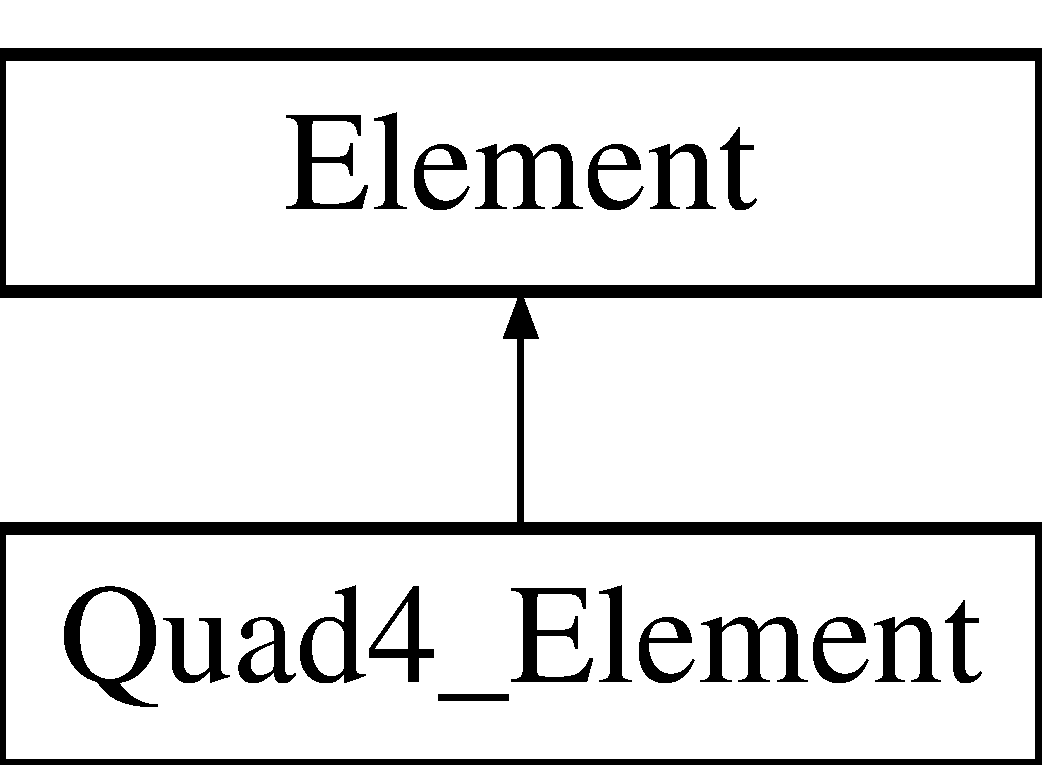
\includegraphics[height=2.000000cm]{class_quad4___element}
\end{center}
\end{figure}
\subsection*{Public Member Functions}
\begin{DoxyCompactItemize}
\item 
\mbox{\hyperlink{class_quad4___element_ac07432e0180b75c6acb534e2327950a7}{Quad4\+\_\+\+Element}} ()
\item 
\mbox{\Hypertarget{class_quad4___element_a6fa23c1b93f10c991b2155f764aa6d19}\label{class_quad4___element_a6fa23c1b93f10c991b2155f764aa6d19}} 
void {\bfseries cal\+\_\+ke} ()
\end{DoxyCompactItemize}
\subsection*{Additional Inherited Members}


\subsection{Detailed Description}


Definition at line 25 of file Quad4\+\_\+\+Element.\+h.



\subsection{Constructor \& Destructor Documentation}
\mbox{\Hypertarget{class_quad4___element_ac07432e0180b75c6acb534e2327950a7}\label{class_quad4___element_ac07432e0180b75c6acb534e2327950a7}} 
\index{Quad4\+\_\+\+Element@{Quad4\+\_\+\+Element}!Quad4\+\_\+\+Element@{Quad4\+\_\+\+Element}}
\index{Quad4\+\_\+\+Element@{Quad4\+\_\+\+Element}!Quad4\+\_\+\+Element@{Quad4\+\_\+\+Element}}
\subsubsection{\texorpdfstring{Quad4\+\_\+\+Element()}{Quad4\_Element()}}
{\footnotesize\ttfamily Quad4\+\_\+\+Element\+::\+Quad4\+\_\+\+Element (\begin{DoxyParamCaption}{ }\end{DoxyParamCaption})}

Default constructor 

Definition at line 8 of file Quad4\+\_\+\+Element.\+cc.


\begin{DoxyCode}
9 \{
10 \}
\end{DoxyCode}


The documentation for this class was generated from the following files\+:\begin{DoxyCompactItemize}
\item 
include/Quad4\+\_\+\+Element.\+h\item 
src/Quad4\+\_\+\+Element.\+cc\end{DoxyCompactItemize}

\hypertarget{classxind}{}\section{xind$<$ T $>$ Class Template Reference}
\label{classxind}\index{xind$<$ T $>$@{xind$<$ T $>$}}
\subsection*{Public Member Functions}
\begin{DoxyCompactItemize}
\item 
\mbox{\Hypertarget{classxind_a03541f9baa82fbd0c237678ab9e64f93}\label{classxind_a03541f9baa82fbd0c237678ab9e64f93}} 
{\bfseries xind} (T x, long ind)
\item 
\mbox{\Hypertarget{classxind_a98331d26bf395e5e2c7df29eb7d61f97}\label{classxind_a98331d26bf395e5e2c7df29eb7d61f97}} 
bool {\bfseries operator$<$} (\mbox{\hyperlink{classxind}{xind}} const \&other) const
\end{DoxyCompactItemize}
\subsection*{Public Attributes}
\begin{DoxyCompactItemize}
\item 
\mbox{\Hypertarget{classxind_a00fdccd018f160800da21a8396c64ba4}\label{classxind_a00fdccd018f160800da21a8396c64ba4}} 
T {\bfseries x}
\item 
\mbox{\Hypertarget{classxind_aa04e6ef061b2ea406bd5c3b22d50261e}\label{classxind_aa04e6ef061b2ea406bd5c3b22d50261e}} 
long {\bfseries ind}
\end{DoxyCompactItemize}


\subsection{Detailed Description}
\subsubsection*{template$<$class T$>$\newline
class xind$<$ T $>$}



Definition at line 8 of file Eig\+Lab.\+h.



The documentation for this class was generated from the following file\+:\begin{DoxyCompactItemize}
\item 
include/Eig\+Lab.\+h\end{DoxyCompactItemize}

%--- End generated contents ---

% Index
\backmatter
\newpage
\phantomsection
\clearemptydoublepage
\addcontentsline{toc}{chapter}{Index}
\printindex

\end{document}
